\pdfminorversion=4
\documentclass[aspectratio=169]{beamer}

\mode<presentation>
{
  \usetheme{default}
  \usecolortheme{default}
  \usefonttheme{default}
  \setbeamertemplate{navigation symbols}{}
  \setbeamertemplate{caption}[numbered]
  \setbeamertemplate{footline}[frame number]  % or "page number"
  \setbeamercolor{frametitle}{fg=white}
  \setbeamercolor{footline}{fg=black}
} 

\usepackage[english]{babel}
\usepackage[utf8x]{inputenc}
\usepackage{tikz}
\usepackage{courier}
\usepackage{array}
\usepackage{bold-extra}
\usepackage{minted}
\usepackage[thicklines]{cancel}
\usepackage{fancyvrb}
\usepackage{tabto}

\xdefinecolor{dianablue}{rgb}{0.18,0.24,0.31}
\xdefinecolor{darkblue}{rgb}{0.1,0.1,0.7}
\xdefinecolor{darkgreen}{rgb}{0,0.5,0}
\xdefinecolor{darkgrey}{rgb}{0.35,0.35,0.35}
\xdefinecolor{darkorange}{rgb}{0.8,0.5,0}
\xdefinecolor{darkred}{rgb}{0.7,0,0}
\definecolor{darkgreen}{rgb}{0,0.6,0}
\definecolor{mauve}{rgb}{0.58,0,0.82}

\xdefinecolor{lightblue}{rgb}{0,0.25,1.0}

\title[2018-09-10-rootworkshop-vectorized-nested]{Vectorized Processing of Nested Data}
\author[shortname]{\textcolor{darkblue}{Jim Pivarski}\inst{a} \and Jaydeep Nandi\inst{b} \and David Lange\inst{a}}
\institute[shortinst]{\inst{a} Princeton University \and \inst{b} National Institute of Technology, Silchar, India}
\date{September 10, 2018}

\usetikzlibrary{shapes.callouts}

\begin{document}

\logo{\pgfputat{\pgfxy(0.11, 7.4)}{\pgfbox[right,base]{\tikz{\filldraw[fill=dianablue, draw=none] (0 cm, 0 cm) rectangle (50 cm, 1 cm);}\mbox{\hspace{-8 cm}
\includegraphics[height=1 cm]{princeton-logo-long.png}
\includegraphics[height=1 cm]{diana-hep-logo-long.png}}}}}

\begin{frame}
  \titlepage
\end{frame}

\logo{\pgfputat{\pgfxy(0.11, 7.4)}{\pgfbox[right,base]{\tikz{\filldraw[fill=dianablue, draw=none] (0 cm, 0 cm) rectangle (50 cm, 1 cm);}\mbox{\hspace{-8 cm}
\includegraphics[height=1 cm]{princeton-logo.png}
\includegraphics[height=1 cm]{diana-hep-logo.png}}}}}

% Uncomment these lines for an automatically generated outline.
%\begin{frame}{Outline}
%  \tableofcontents
%\end{frame}

% START START START START START START START START START START START START START

\begin{frame}{Intersection of three topics}
\vspace{0.5 cm}
\begin{block}{Hardware vectorization}
Single Instruction, Multiple Data (SIMD); primary mode of parallelization on GPUs, only way to fully exploit CPUs that have wide vector registers (e.g.\ AVX-512).
\end{block}

\vspace{0.5 cm}
\uncover<2->{\begin{block}{Array programming}
High-level programming interface with the same structure as SIMD (Single \underline{\it VM} Instruction, Multiple Data), which may or may not be vectorized in hardware.
\end{block}}

\vspace{0.5 cm}
\uncover<3->{\begin{block}{Operations on nested data structures}
Often hard to vectorize or even express with array programming.
\end{block}}
\end{frame}

\begin{frame}[fragile]{Examples of physics problems involving nested data operations}
\vspace{0.15 cm}
\begin{enumerate}
\item Compute the $\phi$ difference between each jet and its event's MET.
\small
\begin{minted}{python}
for event in dataset:
    for jet in event.jets:
        jet.phidiff = jet.phi - event.phi
\end{minted}
\normalsize

\vspace{0.1 cm}
\item<2-> Compute mass of all particles from two collections, subjet to a cut.
\small
\begin{minted}{python}
for event in dataset:
    event.leptoquarks = []
    for jet in event.jets:
        for lepton in event.leptons:
            if cut(jet, lepton):
                event.pairs.append(mass(jet, lepton))
\end{minted}
\normalsize

\vspace{0.1 cm}
\item<3-> Find the ``best'' candidate per event or per subcollection.
\small
\begin{minted}{python}
for event in dataset:
    event.best = None
    for leptoquark in leptoquarks:
        if event.best is None or \
            quality(leptoquark) > quality(event.best):
                event.best = leptoquark
\end{minted}
\normalsize
\end{enumerate}
\end{frame}

\begin{frame}[fragile]{Array programming}
\vspace{0.2 cm}
\hfill 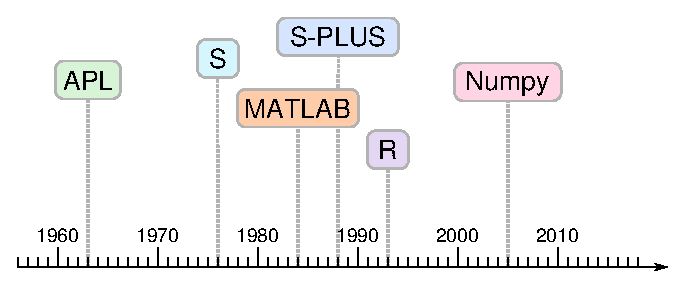
\includegraphics[height=2.75 cm]{apl-timeline.pdf}

\vspace{-2.15 cm}
{\bf\large Long history; not just Numpy}

\vspace{0.5 cm}
Expresses regular operations over \\ rectangular data structures in shorthand.

\vspace{0.25 cm}
\begin{itemize}\setlength{\itemsep}{0.15 cm}
\item<2-> Multidimensional slices: \tabto{5.5 cm}{\small \mintinline{python}{rgb_pixels[0, 50:100, ::3]}}
\item<3-> Elementwise operations: \tabto{5.5 cm}{\small \mintinline{python}{all_pz = all_pt * sinh(all_eta)}}
\item<4-> Broadcasting: \tabto{5.5 cm}{\small \mintinline{python}{all_phi - 2*pi}}
\item<5-> Masking (list compaction): \tabto{5.5 cm}{\small \mintinline{python}{data[trigger & (pt > 40)]}}
\item<6-> Fancy indexing (gather/scatter): \tabto{5.5 cm}{\small \mintinline{python}{all_eta[argsort(all_pt)]}}
\item<7-> Row/column commutativity \tabto{5.5 cm}{\small \mintinline{python}{table["column"][7]} (row 7 of column array)}

(hides AoS $\leftrightarrow$ SoA): \tabto{5.5 cm}{\small \mintinline{python}{table[7]["column"]} (field of row tuple 7)}
\item<8-> Array reduction: \tabto{5.5 cm}{\small \mintinline{python}{array.sum()}} $\to$ scalar
\end{itemize}
\end{frame}

\begin{frame}[fragile]{Extension to variable-sized, nested structures}
\vspace{0.5 cm}
Logical structure: \tabto{3 cm}{\ttfamily\textcolor{black}{[\textcolor{red}{[}\textcolor{darkblue}{0, 1, 2}], \textcolor{red}{[}], \textcolor{red}{[}\textcolor{darkblue}{3, 4}], \textcolor{red}{[}\textcolor{darkblue}{5, 6, 7, 8, 9}]\textcolor{red}{]}}}

\vspace{0.05 cm}
Offsets:           \tabto{3 cm}{\ttfamily\verb|[|\textcolor{red}{0,}\verb|         |\textcolor{red}{3,}\verb|  |\textcolor{red}{3,}\verb|      |\textcolor{red}{5,}\verb|             |\textcolor{red}{10}\verb|]|}

\vspace{0.05 cm}
Content:           \tabto{3 cm}{\ttfamily\verb|[ |\textcolor{darkblue}{0, 1, 2}\verb|,       |\textcolor{darkblue}{3, 4}\verb|,   |\textcolor{darkblue}{5, 6, 7, 8, 9}\verb|]|}

\vspace{0.05 cm}
Parents:           \tabto{3 cm}{\ttfamily\verb|[ |\textcolor{darkgreen}{0, 0, 0}\verb|        |\textcolor{purple}{2, 2,}\verb|   |\textcolor{darkorange}{3, 3, 3, 3, 3}|\verb|]|}

\vspace{0.5 cm}
\uncover<2->{A ``jagged array'' (content $+$ offsets and/or content $+$ parents) is a basic building block of variable-sized, nested structure.}

\begin{itemize}
\item<3-> use a jagged array as the content of another jagged array to get {\tt\small list<list<X>>}
\item<4-> use a fixed-size rectangular array of dimension {\tt\small N} as content to get {\tt\small list<X[N]>}
\item<5-> use a fixed-size rectangular array of dimension {\tt\small M} as offsets to get {\tt\small list<X>[M]}
\end{itemize}

\vspace{0.25 cm}
\uncover<6->{When combined with a table type (column names $\to$ arrays), this is as expressive as any combination of {\tt\small std::vector} and {\tt\small struct} (i.e.\ as expressive as ProtoBuf).}
\end{frame}

\begin{frame}{Array programming can be extended to jagged arrays}
\vspace{0.1 cm}
\begin{columns}
\column{1.05\linewidth}
\begin{itemize}\setlength{\itemsep}{0.15 cm}
\item Multidimensional slices: \tabto{5.5 cm}{\small \mintinline{python}{events["jets"][:, 0]}} $\to$ first jet per event
\item<2-> Elementwise operations: \tabto{5.5 cm}{\small \mintinline{python}{jetpt * sinh(jeteta)}} $\to$ \mbox{keep jagged structure\hspace{-1 cm}}
\item<3-> Broadcasting: \tabto{5.5 cm}{\small \mintinline{python}{jetphi - metphi}} $\to$ expand {\small \mintinline{python}{metphi}} from

\tabto{5.5 cm}one-per-event to one-per-jet before operation

\item<4-> Masking (list compaction): \tabto{5.5 cm}{\small \mintinline{python}{data[trigger]}} $\to$ drop whole events

\tabto{5.5 cm}{\small \mintinline{python}{data[jetpt > 40]}} $\to$ drop jets from events

\item<5-> Fancy indexing (gather/scatter): \tabto{5.5 cm}{\small \mintinline{python}{a = argmax(jetpt)}} $\to$ \mbox{\small \mintinline{python}{[[2], [], [1], [4]]}\hspace{-0.5 cm}}

\tabto{5.5 cm}{\small \mintinline{python}{jeteta[a]}} $\to$ \mbox{\small \mintinline{python}{[[3.6], [], [-1.2], [0.4]]}\hspace{-0.5 cm}}

\item<6-> Row/column commutativity \tabto{5.5 cm}{\small \mintinline{python}{events["jets"]["pt"][7, 1]}} \mbox{(all the same)\hspace{-0.5 cm}}

(project jagged tables to \tabto{5.5 cm}{\small \mintinline{python}{events["jets"][7]["pt"][1]}}

jagged arrays before indexing): \tabto{5.5 cm}{\small \mintinline{python}{events[7]["jets"]["pt"][1]}}

\tabto{5.5 cm}{\small \mintinline{python}{events["jets"][7, 1]["pt"]}}

\tabto{5.5 cm}{\small \mintinline{python}{events[7]["jets"][1]["pt"]}}

\item<7-> Jagged array reduction: \tabto{5.5 cm}{\small \mintinline{python}{jetpt.max()}} $\to$ array of max jet $p_T$ per event
\end{itemize}
\end{columns}
\end{frame}

\begin{frame}[fragile]{Solving physics problems with jagged array programming}
\vspace{0.5 cm}
{\bf Problem 1:} Compute the $\phi$ difference between each jet and its event's MET.
\small
\begin{minted}{python}
for event in dataset:
    for jet in event.jets:
        jet.phidiff = jet.phi - event.phi
\end{minted}
\normalsize

\vspace{0.5 cm}
{\bf Jagged array solution:} 
\small
\begin{minted}{python}
# because of extended broadcasting rules
events["jets"]["phidiff"] = \
    events["jets"]["phi"] - events["MET"]["phi"]
\end{minted}
\end{frame}

\begin{frame}[fragile]{Solving physics problems with jagged array programming}
\vspace{0.5 cm}
{\bf Problem 2:} Compute mass of all particles from two collections, subjet to a cut.
\small
\begin{minted}{python}
for event in dataset:
    event.leptoquarks = []
    for jet in event.jets:
        for lepton in event.leptons:
            if cut(jet, lepton):
                event.pairs.append(mass(jet, lepton))
\end{minted}
\normalsize

\vspace{0.5 cm}
{\bf Jagged array solution:} 
\small
\begin{minted}{python}
# jagged cross-join makes (jet, lepton) pairs per event
pairs = events["jets"].cross(events["leptons"])

events["leptoquarks"] = mass(pairs[cut(pairs)])
\end{minted}
\end{frame}

\begin{frame}[fragile]{Jagged cross-join has a fully vectorizable implementation (Jaydeep)}
\small
\vspace{0.2 cm}

\hfill \mbox{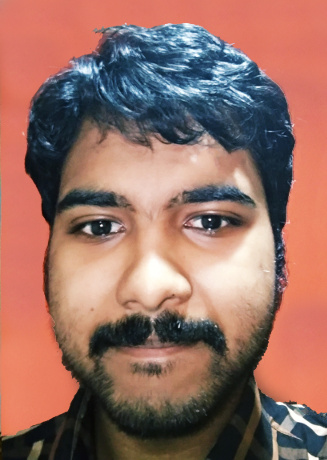
\includegraphics[height=2.5 cm]{jaydeep.jpg}\hspace{-0.75 cm}}

\vspace{-2.7 cm}
\begin{columns}
\column{1.05\linewidth}
\begin{minted}{python}
def cross(self, other):
    offsets = counts2offsets(self.counts * other.counts)
    parents = offsets2parents(offsets)
    indexes = numpy.arange(offsets[-1], dtype=int)

    # fancy indexing get -> SIMD gather
    pi = parents[indexes]
    opi = offsets[pi]
    ocpi = other.counts[pi]

    left = self.offsets[pi][:-1] + ((indexes - opi) // ocpi)
    right = other.offsets[pi][:-1] + (indexes - opi) - (
                                       ocpi * ((indexes - opi) // ocpi))

    return JaggedArray.fromoffsets(offsets, Table(left, right))
\end{minted}
\end{columns}

\normalsize
\vspace{0.5 cm}
(There's also a solution for non-repeating pairs of a collection with itself.)
\end{frame}

\begin{frame}[fragile]{Solving physics problems with jagged array programming}
\vspace{0.25 cm}
{\bf Problem 3:} Find the ``best'' candidate per event or per subcollection.
\small
\begin{minted}{python}
for event in dataset:
    event.best = []
    for leptoquark in leptoquarks:
        if event.best == [] or \
            quality(leptoquark) > quality(event.best[0]):
                event.best = [leptoquark]
\end{minted}
\normalsize

\vspace{0.5 cm}
{\bf Jagged array solution:} 
\small
\begin{minted}{python}
# jagged argmax makes empty lists [] or singleton lists [N]
argbest = quality(events["leptoquarks"]).argmax()

# jagged fancy indexing transforms [] -> [] and [i] -> [sublist[i]]
events["best"] = events["leptoquarks"][argbest]
\end{minted}

\vspace{0.05 cm}
\begin{uncoverenv}<2->
\begin{minted}{python}
# drop empty lists and concatenate by ignoring offsets
nonempty_best = events["best"].flatten()
\end{minted}
\end{uncoverenv}
\end{frame}

\begin{frame}{Surprisingly, jagged reducers are fully vectorizable, too (Jaydeep)}
\only<1>{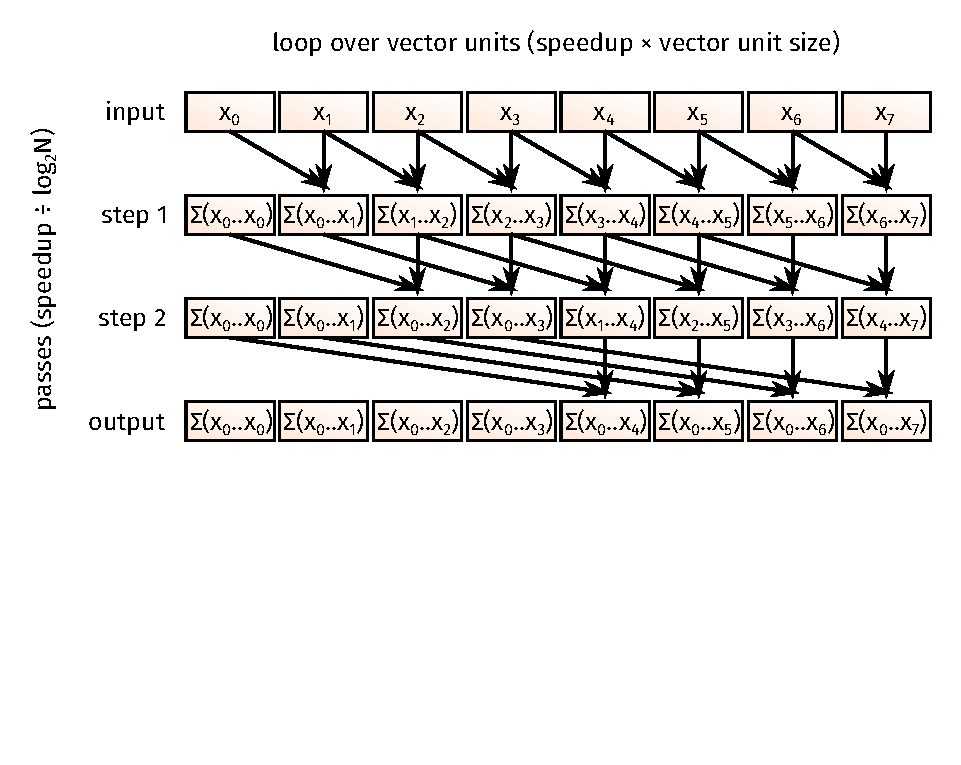
\includegraphics[width=0.75\linewidth]{hillis-steele.pdf}}
\only<2>{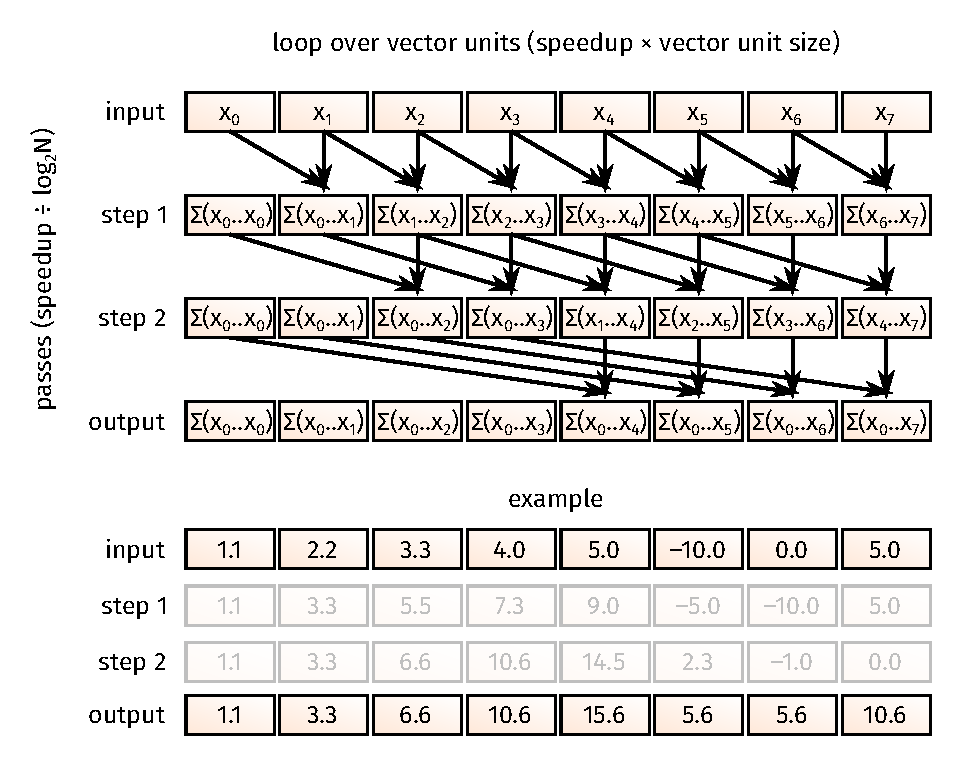
\includegraphics[width=0.75\linewidth]{hillis-steele-2.pdf}}
\only<3>{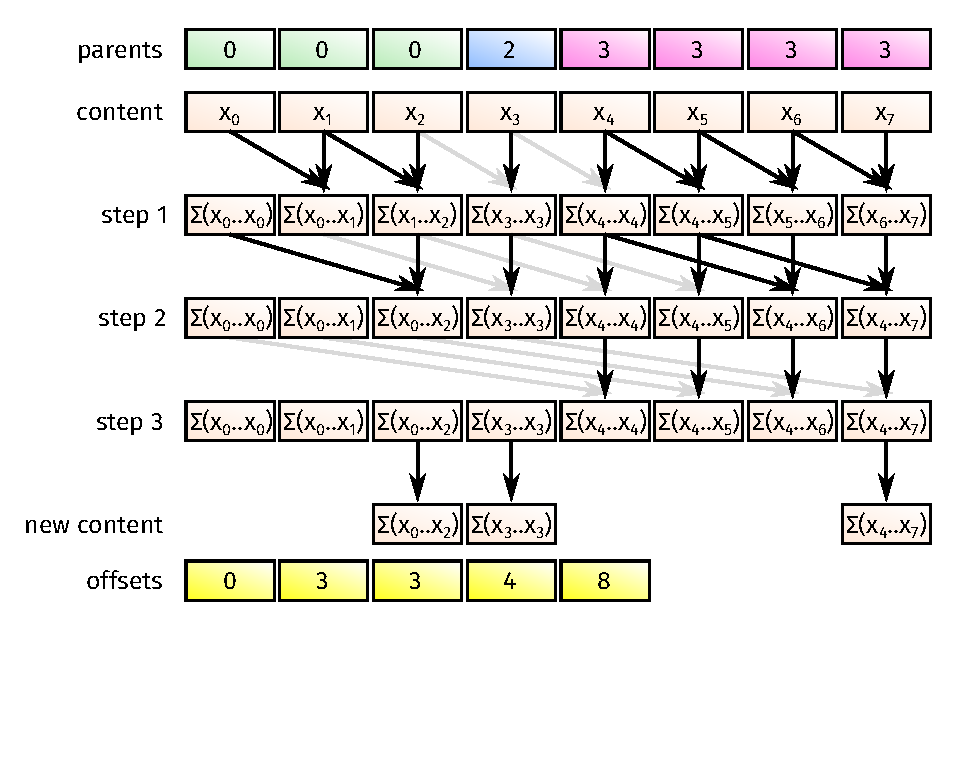
\includegraphics[width=0.75\linewidth]{hillis-steele-3.pdf}}

\only<1>{\vspace{-3 cm} This is known as the Hillis-Steele algorithm: creates a cumulative sum in parallel. \vspace{3 cm}}
\only<3>{\vspace{-1.5 cm} Modification of the Hillis-Steele algorithm: only combine pairs in the same event \\ (by checking parents) and then take the last value in each event. \vspace{1.5 cm}}
\end{frame}

\begin{frame}{Performance of modified Hillis-Steele}
\begin{center}
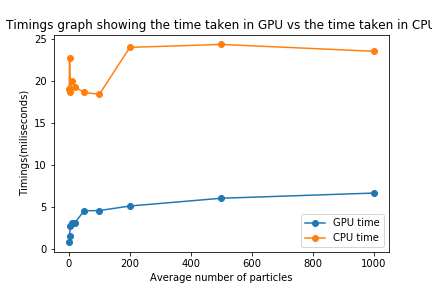
\includegraphics[width=0.5\linewidth]{jagged_max.png}
\end{center}

\textcolor{darkorange}{``CPU time''} is {\tt\small numpy.max.reduceat}, which is a for loop (loop-carried dependency), written in C, executed on a single thread on a Xeon E5-2686.

\vspace{0.15 cm}
\textcolor{lightblue}{``GPU time''} is the new algorithm, written in CUDA, executed on a Tesla K80.

\vspace{0.15 cm}
\textcolor{gray}{\small (TODO: replicate Jaydeep's results, write pure C code (no Numpy), and try to auto-vectorize the new algorithm in CPU.)}
\end{frame}

\begin{frame}{Relevance to ROOT (my conclusions slide)}
\large
\vspace{0.5 cm}
\textcolor{darkblue}{\Large None of the preceeding needs to be in Python or Numpy.}

\vspace{0.5 cm}
\uncover<2->{It was motivated to bypass Python's slow for loops, but it helps physicists express analysis code more succinctly (interface) and it sets up their analysis code for hardware parallelization (performance).}

\vspace{0.5 cm}
\begin{itemize}
\item<3-> The jagged array structure aligns perfectly with the RForest concept.
\item<4-> An array programming model could be supported by the RTensor project.
\item<5-> VecOps::RVec provides one-in-one-out vectorization; it could be extended to provide vectorized jagged operations as well.
\item<6-> Doing so would provide a ``C++ story'' for how physicists can use BulkIO.
\end{itemize}
\end{frame}

\end{document}
